%\documentclass[twocolumn]{article}

\documentclass[]{IEEEtran}

% \documentclass[manuscript, review, screen]{acmart}
% \documentclass[sigconf]{acmart}   % For double column 
% \include{setups/ACMsetup}

%instructions for using setup.tex
\def\mode{0}  %Document (appearance) Mode. part of setup: 
   %0=proofread (to do note comments and color texts stay)
   %1=draft watermark, (comments and colors are eliminated)
   %2=confidential watermark, (comments and colors are eliminated) 
   %3=Pre-publication watermark, (comments and colors are eliminated) 
   %4=final (comments and colors are eliminated,         confidential data is removed    \begin{conf} conf data \end{conf})

\def\redactionmode{2} %redaction mode: 0=none, i=redaction level i (upto4)
   % 0: Nothing is redacted.
   % 1: (2Detailed) Too Much Details
   % 2: (Uncritical) Information that is not very important but it could be there, space permitting
   % 3: (2SaveSpace) Information that is rather relevant/important but could be deleted if short of space
   % 4: (IfMustDelete) Information that is important but can be dropped in extreme cases of limited space
   %\begin{RedactionName} TEXT \end{RedactionName}   for different redaction of Text (RedactionName is one of the 4 above, 2Detailed, Uncritical, etc.)
	 % Please make sure that \begin and \end comment are not indented
	 % moreover, there should be an enter after the command and no comment

\def\alttextmode{1} %alternative text mode mode: 0=A&B, 1:not A & B, 2:A & not B, 3:Not A & Not B
                    %\begin{TextA} \end{TextA}: Alternative Text A 
                    %\begin{TextB} \end{TextB}: Alternative Text B
\include{setups/setup}


%acronyms bank
\include{setups/acronyms}
\include{acronyms_local}

\usepackage{amssymb} % Für das \checkmark-Symbol
\usepackage{booktabs}
\usepackage{amsmath}
\usepackage{svg}

%%%%%%%%%%%%%%%%%%%%%%%%%%%%%%%%%%%%%%%%%%%%%%%%%%%%%%%%%%%%%%%%%%%%%%%%%%%%%%%%%%%%%%%%%%%%%%%%
%%%%%%%%%%%%%%%%%%%%%%%%%%%%%%%%%%%%%%%%%%%%%%%%%%%%%%%%%%%%%%%%%%%%%%%%%%%%%%%%%%%%%%%%%%%%%%%%

\begin{document}
%\bstctlcite{IEEEexample:BSTcontrol}     %Automatic truncating of the list of authors in IEEE template
\title{An IMPLY-based Semi-Parallel Approximate In-Memristor Adder\\
Final Project: Emerging Computing Paradigms WS23}

\author{Constantin Nicolai, Florian Schrittwieser, Malte Bauer}

%%%%%%%%%%%%%%%%% IEEE Authors' information %%%%%%%%%%%%%%%%%%%%%%%%%%
%\author{
%\IEEEauthorblockN{
%N. TaheriNejad (c)\IEEEauthorrefmark{1}, and 
%A. B\IEEEauthorrefmark{2},
%}
%
%\IEEEauthorblockA{
%\IEEEauthorrefmark{1}
%TU Wien, Vienna, Austria\\
%{E-mail:} \{nima.taherinejad, d.r\}@tuwien.ac.at  
%}
%
%\IEEEauthorblockA{
%\IEEEauthorrefmark{2}
%University of Bordeaux INP, Bordeaux, France \\
%{E-mail:} a@b.com
%}
%}
%%%%%%%%%%%%%%%%% End of IEEE Authors' information %%%%%%%%%%%%%%%%%%%


%%%%%%%%%%%%%%%%% ACM Authors' information %%%%%%%%%%%%%%%%%%%%%%%%%%

% %\titlenote{Footnote for title}

% \author{N. TaheriNejad}
% \orcid{0000-0002-1295-0332}
% \authornote{A common footnote.}
% \affiliation{
%   \institution{TU Wien}
%   \department{Institute of Computer Technology}
%   \streetaddress{Gusshausstrasse 25-27}
%   \city{Vienna}
%   \postcode{1040}
%   \country{Austria}
%   }
% \email{nima.taherinejad@tuwien.ac.at}

% \author{D. R.}
% \orcid{0000-0000-0000-0000}
% \authornotemark[2]
% \authornote{Individual footnote.}
% \affiliation{}
% \email{}

% %\renewcommand\shortauthors{TaheriNejad et al}

%%%%%%%%%%%%%%%%% End of ACM Authors' information %%%%%%%%%%%%%%%%%^^

\maketitle


\begin{abstract}
% This template provides features for easy switch between draft version, confidential, and final versions. It also provides means for applying different levels of redaction (including an alternative text mode) to adaptively and quickly change the text length. It has an extensive set of acronyms already defined and for colored text commands you can use red, blue, green (with a slash in the beginning). Many useful packages are already included and any figure inside /figure is automatically found (no need for addressing).\\
% Motivatoion, approach, hw implementation, results, applocatio testing
In the landscape of modern computer engineering the energy wall is our prime concern. We therefore propose a more energy efficient memristor-based approximate semi parallel full adder design. The imply logic based full adder is expanded to an 8-bit ripple carry adder and tested in image processing and machine learning applications. These application tests show our design to perform among the best approximate implementations in terms of energy efficiency and still producing usable results. 
\end{abstract}

\glsresetall

\section{Introduction}
Studies have shown that data movement within computing devices s a significant bottleneck. For example, in mobile systems, 41\% of energy consumption is attributed to data movement during web browsing. Furthermore, 34.6\% of total device energy is expended on transferring data between memory hierarchy levels \cite{6983056}. The underlying problem here is the Von Neumann bottleneck \cite{7878940}. 
%TODO: QUELLEN raussuchen
But beside the Von Neumann bottleneck also the general increase in computing power cannot continue indefinitely as the end of Moors Law, the end of Dennards scaling and Amdahls Law show\cite{7878940, 6689270}. The above-mentioned problems highlight the necessity for emerging new computing methods that address them.
One possibility that seems promising is approximate computing which attempts to reduce computing time, hardware complexity and power consumption by performing calculations less accurately \cite{}.
Approximating calculations can be relevant for error-tolerant applications such as image processing, machine learning and generally for applications with noisy input. Using approximation in these Applications is possible since these exhibit an inherent error tolerance an therby accept inaccurat results and don't need fully exact results \cite{9024190}.\\
Another promising approach to overcome the limitations of increasing computing power is in-memory computing solutions. Instead of spending time and energy moving data back and forth between memory and processor, the IMC approach relies on performing calculations directly at the location where the data is stored. This eliminates the bottleneck of Von Neumann architectures and enables more efficient processing. In addition to the solutions for in-memory computing with DRAM and MRAM, it has been shown that in-memory computing is also possible with memristors \cite{sebastian-2020}.\\
In this paper, a new approximating algorithm based on the stateful logic \gls{imply} is presented based on the semi-parallel memristor full adder topology presented in the work "\textit{A Semiparallel Full-Adder in IMPLY Logic}" by Shokat Ganjeheizadeh Rohani, Nima Taherinejad, and David Radakovits \cite{8832255}. Compared to the exact algorithm for the semi-parallel topology, the number of execution steps and the energy required for the calculation could be reduced with this algorithm. However, the error caused by the approximation must be accepted.
In this paper, the basics and the state of the art are briefly discussed in Section \ref{ch:background}. Section \ref{ch:exactImplyAdders} then presents exact \gls{imply} adders, in particular the semi-parallel topology, followed by a discussion of the approximation algorithm in Section \ref{ch:proposedAPPROX}. Among other things, a simulation of the algorithm at circuit level in LT Spice is presented in this section to verify the approximating algorithm.
In order to evaluate the effects of the error caused by the approximation, the approximating full adder is used in two image processing (Section \ref{ch:APPIMAGE}) and two machine learning (Section \ref{ch:APPML}) applications and the results are compared with other state of the art exact and approximating algorithms.

\section{Background}
\label{ch:background}
  
\subsection{Memristors and stateful logic}
Memristors are regarded as the fourth fundamental component alongside resistors, coils and capacitors. The property that characterizes the memristor is that its electrical resistance can be adjusted by the preceding voltage curve on the memristor. Even if the power supply is interrupted, the resistance set by the voltage curve remains in the memristor. Memristors are therefore particularly suitable for storage applications \cite{memristors} \cite{1083337}. 
The memristor as a component has two connections. The resistance set by the voltage curve can be either minimum ($R_{on}$) or maximum ($R_{off}$). In order to be able to use meristors for binary operations resistance has to be treated as logical states. In previous work it has been conclusively agreed that the maximum resistance of the memristors is regarded as low, or "0", and the minimum resistance as high, or "1" \cite{10305490, 10032497, 9841969, 8832255, 8961312, 7946813}.
New computer architectures can be explored through in-memory calculations. Memristors are ideal for this, as they can store states, perform logical operations and serve as input/output \cite{1083337}. There are a variety of ways to perform calculations and logical functions with memristors \cite{9321508, alam-2022, 9741240, 9382267, 8587724, 6895258, 6331426}. \gls{imply} has stood out in particular, as this stateful logic can be used to perform operations within the crossbar array structure \cite{8388838}. Figure \ref{fig:ImplyGate} shows an \gls{imply} gate consisting of two memristors connected to a resistor $R_G$. In order to perform a logical implication $a \rightarrow b$, a voltage $V_{condt}$ must be applied to memristor $a$ and $V_{set}$ to $b$, the truth table for the implication is in table \ref{tab:ImplyLogicTT}. The inputs are the initial states of the memristors, while the output is in memristor $b$. The initial state in memristor $b$ is overwritten after the memristor threshold voltage is exceeded and is therefore lost. More detailed information on memristors and \gls{imply} is available in \cite{borghetti-2010, 5226356, 6617731, 1083337}.

\begin{figure}[h]
	\centering
	\includegraphics[width=0.4\linewidth]{2023_IEEE_JETCAS_AxCimplyAdder-cropped}
	\caption{Circuit-level memristor based \gls{imply} logic gate \cite{10032497}}
	\label{fig:ImplyGate}
\end{figure}

\begin{table}[h]
\centering
\begin{tabular}{|c|c|c|}
\hline
a & b & b' = a $\rightarrow$ b \\ \hline
\addlinespace[1ex] \hline
0 & 0 & 1                                  \\ \hline
0 & 1 & 1                                  \\ \hline
1 & 0 & 0                                  \\ \hline
1 & 1 & 1                                  \\ \hline
\end{tabular}
\caption{\gls{imply} logic Truth table \cite{10032497}}
\label{tab:ImplyLogicTT}
\end{table}

\subsection{Approximat computing and quality assesment/comparison of the results}
%TODO: @Florian @Nicholai
\section{Imply based adders}
\label{ch:exactImplyAdders}
\subsection{Adder topologies}
Various full adder topologies based on the stateful logic IMPLY already exist. In general, these can be divided into serial, parallel and mixed forms that try to combine the best of the classical topologies such as semi-serial and semi-parallel. An approximating algorithm has already been presented for many of these topologies, which reduces the number of calculation steps and the energy required for an addition by deliberately accepting an error.
A selection of the exact and approximating algorithms and the number of steps and energy required to perform a 1-bit full addition is shown in Table \ref{tab:comparisonBIG} \textbf{a)}. The table also lists the number of errors in the approximating sum bit and the approximating carry bit for the approximating algorithms.

\begin{table*}[]
\centering
\begin{tabular}{|c|c|c|c|c|c|cc|}
\hline
 Nr. &
  Exact designs &
  \begin{tabular}[c]{@{}c@{}}Approximating\\ designs\end{tabular} &
  \begin{tabular}[c]{@{}c@{}}Execution\\ steps\end{tabular} &
  \#Memristors &
  \begin{tabular}[c]{@{}c@{}}\# CMOS\\ Switches\end{tabular} &
  \multicolumn{1}{c|}{\begin{tabular}[c]{@{}c@{}}erroneous\\ sums\end{tabular}} &
  \begin{tabular}[c]{@{}c@{}}erroneous \\ couts\end{tabular} \\ \hline
  \addlinespace[1ex]  
    \multicolumn{8}{l}{\textbf{a)}} \\
    \addlinespace[1ex]  
  \hline
1 &
  Serial \cite{7946813} &
   &
  22n &
  2n+1 &
  0 &
  \multicolumn{2}{c|}{-} \\ \hline
2 &
   &
  Serial \cite{9841969} &
  8n &
  2n+1 &
  0 &
  \multicolumn{1}{c|}{3/8} &
  1/8 \\ \hline
3 &
   &
  Serial (SIAFA1) \cite{10032497} &
  8n &
  2n+1 &
  0 &
  \multicolumn{1}{c|}{3/8} &
  1/8 \\ \hline
4 &
   &
  Serial (SIAFA2) \cite{10032497} &
  10n &
  2n+1 &
  0 &
  \multicolumn{1}{c|}{2/8} &
  1/8 \\ \hline
5 &
   &
  Serial (SIAFA3) \cite{10032497} &
  8n &
  2n+1 &
  0 &
  \multicolumn{1}{c|}{3/8} &
  1/8 \\ \hline
6 &
   &
  Serial (SIAFA4) \cite{10032497} &
  8n &
  2n+1 &
  0 &
  \multicolumn{1}{c|}{3/8} &
  1/8 \\ \hline
7 &
  Semi Serial \cite{8961312} &
   &
  10n+2 &
  2n + 6 &
  12 &
  \multicolumn{2}{c|}{-} \\ \hline
8 &
   &
  Semi Serial \cite{10305490} &
  5 (+ 1  inital) &
  2n+3 &
  12 (6?) &
  \multicolumn{1}{c|}{3/8} &
  1/8 \\ \hline
9 &
  Parallel \cite{karimi-2018} &
   &
  5n+16 &
  4n+1 &
  n &
  \multicolumn{2}{c|}{-} \\ \hline
10 &
  Semi Parallel \cite{8832255} &
   &
  17n &
  2n+3 &
  3 &
  \multicolumn{2}{c|}{-} \\ \hline
  \addlinespace[1ex]  
    \multicolumn{8}{l}{\textbf{b)}} \\
    \addlinespace[1ex]  
  \hline
11 &
   &
  Proposed semi parallel &
  5n &
  2n+3 &
  3 &
  \multicolumn{1}{c|}{3/8} &
  1/8 \\ \hline

\end{tabular}
\caption{Selection of exact and approximate algorithms/topologies, number of execution steps, number of memristors required, number of CMOS switches and erroneous sums/couts for approximate algorithms.}
\label{tab:comparisonBIG}
\end{table*}
%TODO unsere raus nehmen oder drinnenlassen?
%TODO mit Florian und Nicholas durchsprechen

\subsection{Exact semi-parallel adder topology and execution steps}
This paper presents an approximating algorithm based on the semi-parallel full adder presented in the work "\textit{A Semiparallel Full-Adder in IMPLY Logic}" by Shokat Ganjeheizadeh Rohani, Nima Taherinejad, and David Radakovits \cite{8832255}. 
The semi-parallel-adder topology used is shown in Figure \ref{fig:exactFullAdderTopology}. For an n-bit calculation, it consists of 2n input memristors ($a_{n}$ and $b_{n}$), one carry memristor ($c$) and two work memristors ($w_{1}$ and $w_{2}$).  The topology takes advantage of the simple serial connection of the input memristors, but splits them into two serial strings, allowing parallel operations. To enable operations between the two serial strands, they are connected with a switch ($s_{2}$). To enable imply operations between the memristors, each serial chain of memristors must be connected to a resistor $R_G$, as shown in Figure \ref{fig:ImplyGate}. In order for both serial strings to be able to perform operations independently of each other in the semi-parallel topology, both strings must each be provided with an imply load resistor $R_G$. As $R_{G1} \parallel R_{G2}$  is present at the moment that both strands are connected when $s_{2}$ is closed, only half the resistance $R_G/2$ would be present. To ensure that operations can still be carried out, it must be possible to separate both strands from the resistors. As shown in figure \ref{fig:exactFullAdderTopology}, this is made possible by switches $s_1$ and $s_2$.
\begin{figure}[h]
	\centering
	\includegraphics[width=0.8\linewidth]{2020_SemiparallerIMPLYadder_TVLSI_cropped-cropped}
	\caption{Exact semi-parallel full adder topology, presented in \cite{8832255}}
	\label{fig:exactFullAdderTopology}
\end{figure}
\\ The algorithm proposed in the paper for the semi-parallel topology is for a 1 bit full adder. The underlying logic for calculating the Sum (S) and the Carry-out (C$_{out}$) is
\begin{equation}
S = [(\overline{a} \rightarrow b) \rightarrow ((a \rightarrow \overline{b}) \rightarrow c)] \rightarrow (\overline{(\overline{a \oplus b}) \rightarrow \overline{c}})
\end{equation}
\begin{equation}
C_{out} = \overline{(\overline{a} \rightarrow b) \rightarrow \overline{((a \rightarrow \overline{b}) \rightarrow c)}}
\end{equation}
with a, b as the inputs and Carry-in as c. The logic for the sum can be executed in 17 steps, while the logic for the Carry-out can be executed from a intermediate result of the calculation of the sum in two additional steps.
\bigbreak
In summary, the topology for a exact semi-parallel n-bit addition consists of 2n+3 memristors and 3 additional CMOS switches. 1-bit calculations can be performed in 17 steps, thereby allowing for n-bit calculations to be accomplished in 17n steps.

\section{Proposed approximating algorithm for the semi-parallel full adder topology}
\label{ch:proposedAPPROX}

In previous work, \gls{imply}-based approximating algorithms for serial and semi-serial algorithms have already been investigated. As shown in table \ref{tab:comparisonBIG} \textbf{a)} these algorithms require between 5 and 10 steps to calculate the sum and carry bits and have between 2 and 3 erroneous bits of the 8 input options in the sum and one erroneous bit in the carry.
In order to be competitive with these presented algorithms, all combinations of three steps depth of the basic operations FALSE and IMPLY were performed via brute force. Since it should be possible to simply cascade several full adders to a \gls{rca} of size n no changes are to be made to the topology. Furthermore for simple cascading the result of the addition of one bit should be in section one while the carry bit should be in memristor c. Based on these results, it was investigated whether a carry bit can be approximated by a few further operations. It has been shown that a carry with an error of 1/8 can be generated by 1 additional imply and invert operation. One combination in particular stood out, which is carried out in five steps in the semi-parallel topology as shown in Table \ref{tab:procedure_apprxFullAdder} and which fulfils the requirements that the sum remains in Section 1 after calculation and the calculated carry out lies in memristor C. The truth table for the sum and the carry bit resulting from the five computational calculation steps is shown in Table \ref{tab:truthTable}.

\begin{table}[h]
\centering
\caption{\\
Steps for an approximate semi-parallel full adder. A and B are inputs, outputs in A (Sum) and in W2 (C$_{out}$), "1" for a closed and "0" for an opened switch..}
\label{tab:procedure_apprxFullAdder}
\begin{tabular}{|c|cc|c|}
\hline
Steps & \multicolumn{1}{c|}{Section 1} & Section 2 & \begin{tabular}[c]{@{}c@{}}Switches\\ (S1,S2,S3)\end{tabular} \\ \hline \addlinespace[1ex] \hline
1 & \multicolumn{1}{c|}{\textit{w$_{1}$ = 0}} & \textit{w$_{2}$ = 0} & (1,0,1) \\ \hline
2 & \multicolumn{1}{c|}{\textit{a $\rightarrow$ w$_{1}$ = w$_{1}$'}} & \textit{c $\rightarrow$ w$_{2}$ = w$_{2}$'} & (1,0,1) \\ \hline
3 & \multicolumn{2}{c|}{\textit{b $\rightarrow$ w$_{1}$' = w$_{1}$''}} & (0,1,1) \\ \hline
4 & \multicolumn{2}{c|}{\textit{w$_{2}$' $\rightarrow$ w$_{1}$'' = w$_{1}$''' (Result: Sum)}} & (0,1,1) \\ \hline
5 & \multicolumn{2}{c|}{\textit{w$_{1}$''' $\rightarrow$ c = c' (Result: C$_{out}$)}} & (0,1,1) \\ \hline
\end{tabular}
\end{table}

\begin{table}[h]
\centering
\caption{\\The equivalent logic to the procedure shown in Table \ref{tab:procedure_apprxFullAdder}}
\label{tab:my-table3}
\begin{tabular}{|ccc|}
\hline
\multicolumn{3}{|c|}{Equivalent Logic} \\ \hline
\multicolumn{1}{|c|}{Steps} & \multicolumn{1}{c|}{Section 1} & Section 2 \\ \hline \addlinespace[1ex] \hline
\multicolumn{1}{|c|}{1} & \multicolumn{1}{c|}{\textit{$False(w_{1})$}} & \textit{$False(w_{2})$} \\ \hline
\multicolumn{1}{|c|}{2} & \multicolumn{1}{c|}{\textit{$w_{1} = \overline{a}$}} & \textit{$w_{2} = \overline{c}$} \\ \hline
\multicolumn{1}{|c|}{3} & \multicolumn{2}{c|}{\textit{$b \rightarrow \overline{a}$}} \\ \hline
\multicolumn{1}{|c|}{4} & \multicolumn{2}{c|}{\textit{$Sum = w_{1} = \overline{c} \rightarrow (b \rightarrow \overline{a})$}} \\ \hline
\multicolumn{1}{|c|}{5} & \multicolumn{2}{c|}{\textit{$C_{out} = c = (\overline{c} \rightarrow (b \rightarrow \overline{a})) \rightarrow c$}} \\ \hline
\end{tabular}
\end{table}

\begin{table}[h]
\centering
\caption{\\Truth table of approximate algorithm}
\label{tab:truthTable}
\begin{tabular}{|c|c|c|c|c|c|c|}
\hline
A$_{in}$ & B$_{in}$ & C$_{in}$ & \begin{tabular}[c]{@{}c@{}}Exact\\ \textit{Sum}\end{tabular} & \begin{tabular}[c]{@{}c@{}}Exact\\ C$_{out}$\end{tabular} & \begin{tabular}[c]{@{}c@{}}Apprx\\ \textit{Sum}\end{tabular} & \begin{tabular}[c]{@{}c@{}}Apprx\\ C$_{out}$\end{tabular} \\ \hline \addlinespace[1ex] \hline
0 & 0 & 0 & 0 & 0 & 1 X & 0 $\checkmark$ \\ \hline 
0 & 0 & 1 & 1 & 0 & 1 $\checkmark$ & 1 X \\ \hline
0 & 1 & 0 & 1 & 0 & 1 $\checkmark$ & 0 $\checkmark$ \\ \hline
0 & 1 & 1 & 0 & 1 & 1 X & 1 $\checkmark$ \\ \hline
1 & 0 & 0 & 1 & 0 & 1 $\checkmark$ & 0 $\checkmark$ \\ \hline
1 & 0 & 1 & 0 & 1 & 1 X & 1 $\checkmark$ \\ \hline
1 & 1 & 0 & 0 & 1 & 0 $\checkmark$ & 1 $\checkmark$ \\ \hline
1 & 1 & 1 & 1 & 1 & 1 $\checkmark$ & 1 $\checkmark$ \\ \hline
\end{tabular}
\end{table}

\section{CIRCUIT-LEVEL SIMULATIONS AND ERROR METRICS}
%TODO: Der Algorithmus für einen größeren Adder welcher obere Bits exakt und untere approximiert berechnet muss angepasst werden, da das Carry Bit nicht im richtigen Memristor liegt!!!!
%TODO: Verwendetes LTSpice Modell Vteam erwähnen
\subsection{Simulation setup}
To verify the correct functioning of the full adder, the semi-parallel topology was simulated with the approximating algorithm in the LT-SPICE circuit simulation software. To enable comparability with the exact/approximating full adders used in previous work, the same setup was used as in works \cite{7946813, karimi-2018, 10032497, 10305490}. This setups consits of the \gls{vteam} model \cite{7110565} which was used and implemented as a SPICE model in order to be able to use it in LT-SPICE. The necessary parameters selected for the model are shown in Table \ref{tab:setupsandparameter} a). It is noteworthy that these parameters were derived through fitting the model to discrete memristors, resulting in slower operations and higher power consumption compared to integrated devices, akin to the disparity between discrete CMOS devices and their integrated equivalents.
Furthermore, the same IMPLY logic parameters were used, which are shown in tabel \ref{tab:setupsandparameter} b).
\subsection{Results of the simulation}
In the first step of the verification of the presented approximating algorithm for the semi-parallel topology, the circuit was simulated at circuit level with the setup presented above. All eight possible input combinations were applied to the input memristors '$a1$', '$b1$', '$c$' and the output was recorded. The result for the sum is after four steps in the work memristor in section 1 ('$w1$') and the result for the carry out after five steps in the '$c$' memristor (section 2). As each step takes 30µs, the result for the sum is therefore available after 120µs and the result for the $C_{out}$ bit after 150µs. The results obtained in the approximating algorithm for the semi-parallel topology of the first verification step match the truth table presented in Table \ref{tab:truthTable}. A correct calculation for the input case '$a1 = 0$', '$b1 = 1$', '$c = 0$' and an incorrect calculation due to the design for input case '$a1 = 1$', '$b1 = 0$', '$c = 1$' are shown in Figure \ref{fig:input033300} a) and b). 

\begin{table}[h]
\centering
\caption{a) VTEAM setup parameter and b) IMPLY logic parameter}
\setlength{\tabcolsep}{1mm}
\begin{tabular}{|c|c|c|c|c|c|c}
    \multicolumn{7}{l}{\textbf{a)}} \\
    \addlinespace[1ex]  
  \hline 
Parameter & $v_{off}$  & $v_{on}$    & $\alpha_{off}$ & $\alpha_{on}$ & $R_{off}$   & \multicolumn{1}{c|}{$R_{on}$}     \\ \hline
Value     & 0,7V  & -10mV  & 3         & 3       & 1 M$\Omega$ & \multicolumn{1}{c|}{10 k$\Omega$} \\ \hline \addlinespace[1ex] \hline
$k_{on}$       & $k_{off}$  & $w_{off}$   & $w_{on}$       & $w_{C}$       & $\alpha_{off}$   & \multicolumn{1}{c|}{$\alpha_{on}$}     \\ \hline
-0,5 nm/s & 1cm/s & 0 nm   & 3 nm      & 107 pm   & 3 nm   & \multicolumn{1}{c|}{0 nm}    \\ \hline
  \addlinespace[1ex]  
    \multicolumn{7}{l}{\textbf{b)}} \\
    \addlinespace[1ex]  
  \cline{1-6}
Parameter & $V_{SET}$  & $V_{RESET}$ & $V_{COND}$     & $R_{G}$      & $t_{pulse}$ &                              \\ \cline{1-6}
Value     & 1 V   & -1 V   & 900 mV    & 40 k$\Omega$ & 30 $\mu s$  &                              \\ \cline{1-6}
\end{tabular}
\label{tab:setupsandparameter}
\end{table}

\begin{figure}[h]
	\centering
	\includegraphics[width=1\linewidth]{newPlot_cropped}
	\caption{LTspice simulation results: In (a) the correct calculation of the output Sum = 1, Cout = 0 for the input a = 0, b = 1, c = 0 by the approximating full adder. In (b), on the other hand, an incorrect calculation by design with Sum = 1, Cout = 1 for the input a = 1, b = 0, c = 1.}
	\label{fig:input033300}
\end{figure}

In the second step of the verification, the approximating algorithm was concatenated in cascoding to a four-bit fully approximating \gls{rca} and a partially approximating 8-bit \gls{rca}. The partially approximating eight bit \gls{rca} was configured so that the lowest three bits are approximated and the remaining five upper bits are calculated with the exact algorithm. With both concatenations of the approximating algorithm to an \gls{rca}, it must be noted that the result of the sum of one bit is not available in memristor '$a$' after the calculation is complete, as in the exact algorithm, but in the work memristor '$w1$'. In order to make cascading possible, the next stage must therefore fall back on the input memristor of the previous calculation as the new work memristor. This is the Input memristor of the previous calculation that has become free in Section 1 ('$a_{n-1}$') . As this then functions as a work memristor and is written directly to 0 (FALSE) in the first step of the algorithm, the result is not falsified by its previous state. Random input values were applied to the fully and partially approximating RCA and compared with the results of a purely computational model. Both RCAs achieved the expected results. 

\subsection{Analysis of energy consumption and comparison with the exact algorithm}
At circuit level, the LT-SPICE energy consumption tool was used to analyze the energy for the calculation of all eight combinations of the approximating full adder in semi-parallel topology. In addition, the semi-parallel topology \cite{} was set up in LT-Spice at circuit design level and the energy consumption for all 8 input combinations was recorded.
The results are shown in Table \ref{tab:energy}. These show that, on average, the approximated adder requires only 32,9\% of the energy of the exact full adder.

% Please add the following required packages to your document preamble:
% \usepackage{multirow}
\begin{table}[h]
\centering
\begin{tabular}{|ccccc|c|}
\hline
\multicolumn{3}{|c|}{Input}                                               & \multicolumn{2}{c|}{Energy}          & \multirow{2}{*}{Efficiency difference (\%)} \\ \cline{1-5}
\multicolumn{1}{|c|}{a} & \multicolumn{1}{c|}{b} & \multicolumn{1}{c|}{c} & \multicolumn{1}{c|}{Exact {[}pJ{]}} & Approx {[}pJ{]} &  \\ \hline \addlinespace[1ex] \hline
\multicolumn{1}{|c|}{0} & \multicolumn{1}{c|}{0} & \multicolumn{1}{c|}{0} & \multicolumn{1}{c|}{2068,7} & 696,69 & 33,7                                        \\ \hline
\multicolumn{1}{|c|}{0} & \multicolumn{1}{c|}{0} & \multicolumn{1}{c|}{1} & \multicolumn{1}{c|}{1962,8} & 661,61 & 33,7                                        \\ \hline
\multicolumn{1}{|c|}{0} & \multicolumn{1}{c|}{1} & \multicolumn{1}{c|}{0} & \multicolumn{1}{c|}{1853,7} & 641,68 & 34,6                                        \\ \hline
\multicolumn{1}{|c|}{0} & \multicolumn{1}{c|}{1} & \multicolumn{1}{c|}{1} & \multicolumn{1}{c|}{1797,8} & 611,95 & 34,0                                        \\ \hline
\multicolumn{1}{|c|}{1} & \multicolumn{1}{c|}{0} & \multicolumn{1}{c|}{0} & \multicolumn{1}{c|}{1982,9} & 642,26 & 32,4                                        \\ \hline
\multicolumn{1}{|c|}{1} & \multicolumn{1}{c|}{0} & \multicolumn{1}{c|}{1} & \multicolumn{1}{c|}{1893,6} & 612,56 & 32,3                                        \\ \hline
\multicolumn{1}{|c|}{1} & \multicolumn{1}{c|}{1} & \multicolumn{1}{c|}{0} & \multicolumn{1}{c|}{1882}   & 581,57 & 30,9                                        \\ \hline
\multicolumn{1}{|c|}{1} & \multicolumn{1}{c|}{1} & \multicolumn{1}{c|}{1} & \multicolumn{1}{c|}{1811,2} & 568,23 & 31,4                                        \\ \hline \addlinespace[1ex] \hline
\multicolumn{5}{|r|}{\textbf{Mean}}                                                                              & \textbf{32,9}                               \\ \hline
\end{tabular}
\caption{Energy consumption of the exact and approximated algorithm for all input combinations. Furthermore, the proportion of energy consumption of the approximating algorithm in relation to the exact algorithm for all combinations and the mean value over all combinations.}
\label{tab:energy}
\end{table}

\subsection{Comparison of execution time and area usage of exact and approximating algorithms for IMPLY full adders}
In order to be able to make a statement about the performance of the proposed approximating algorithm, it is briefly compared with the exact semi parallel and \gls{soa} apporximating full adders in terms of execution time and area usage. Regarding the approximating algorithms the comparison is only carried out with the approximating full adders presented in \cite{10305490, 7946813, 10032497}, as these also use IMPLY logic. We have refrained from a comparison with other approximating adders, as there are considerable differences here that would make any comparison less meaningful. The brief comparison is shown in table \ref{tab:comparisonBIG} a and b. 
\subsubsection{Execution time}
As can be seen from the table, the proposed approximating algorithm requires 5n steps per bit compared to 17n steps required by the exact algorithm in the semi-parallel topology and thus only ~29.4\% of the computation time. A comparison of the proposed algorithm with other soa approximating adders shows that it requires the same number of execution steps as the Approximating Semi Serial Algorithm and about 62.5\% of the execution steps of the Approximating Serial Algorithms.

\subsubsection{Area usage}

%TODO: SChauen, dass oben kklar hervorgeht, dass ich nur innerhlab fas vergleiche.
%TODO: Accuraccy besser einbinden
%TODO: Energy Consumption besser reinnehmen

%Locking at Figure \ref 

%%% FLORIAN %%%
\subsection{Error analysis}
To evaluate the circuit, an 8-bit \gls{rca} was set up and simulated in Python. The qualitative evaluation was carried out using \gls{med}, \gls{nmed} and \gls{mred} metrics. Bit approximation was carried out upwards from LSB, more information can be found in \cite{9271703}. All possible combinations in 8 bits were selected as data for the calculation. With reference to the data shown in Table \ref{tab:errorAnalysis}. It should be noted that successive approximation levels in the range from 1/8 to 4/8 bit for the error metrics MED and NMED result in a tripling of the error per level. For the range from 5/8 to 8/8 bit, the error increase flattens to doubling.
\begin{table}[h]
\caption{Error Metrics of the algorithm in a 8-bit RCA with different approximation degrees}
\centering
\begin{tabular}{|p{1.5cm}|c|c|c|}
\hline
 Approximated Algorithm & \multicolumn{1}{|c|}{\multirow{2}{*}{MED}} & \multicolumn{1}{|c|}{\multirow{2}{*}{NMED}} & \multicolumn{1}{|c|}{\multirow{2}{*}{MRED}}  \\ \hline
 \multicolumn{4}{|c|}{8-bit  RCA} \\ \hline \addlinespace[1ex] \hline
 Ax: 1/8 & 0.25 & 0.00098 & 0.002 \\ \hline
 Ax: 2/8 & 1.13 & 0.00442 & 0.00881 \\ \hline
 Ax: 3/8 & 3.45 & 0.01355 & 0.0267 \\ \hline
 Ax: 4/8 & 9.0 & 0.03529 & 0.06852 \\ \hline
 Ax: 5/8 & 21.53 & 0.08444 & 0.15913 \\ \hline
 Ax: 6/8 & 48.67 & 0.19086 & 0.33934 \\ \hline
 Ax: 7/8 & 101.33 & 0.39735 & 0.63969 \\ \hline
 Ax: 8/8 & 148.56 & 0.58257 & 0.86519 \\ \hline
\end{tabular}
\label{tab:errorAnalysis}
\end{table}

Comparing our own quality metrics to other published approximated \gls{rca} Figure \ref{fig:MED comparison} it is visible that the error for our \gls{rca}, especially with increasing approximation level increases much faster. Taking a look at the truth table at Table \ref{tab:truthTable} it can be seen that for the sum, there is only one case where the approximated sum is zero. At this specific entry in the truth table the approximated carry is one, this leads to the fact that in the next computational step the sum must be again one. This results in a carry that is taking into account as a \gls{msb} boosting the error metrics especially for increasing approximation level.

\begin{figure}[h]
	\centering
	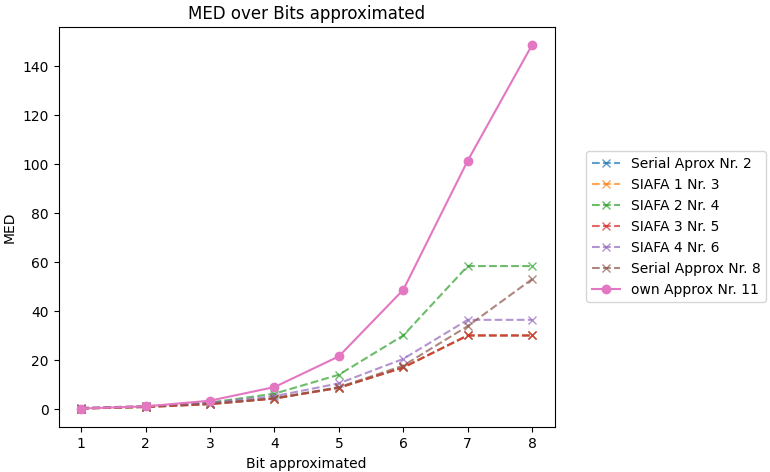
\includegraphics[width=1\linewidth]{figures/erroremtricMED.png}
	\caption{\gls{MED} in comparison to other approximation algorithms}
	\label{fig:MED comparison}
\end{figure}

\newpage

\section{Application in image processing}
\label{ch:APPIMAGE}
Image processing is a widespread technology that is used in industries such as medicine or manufacturing. The simulation is implemented using Python. The qualitative evaluation of the algorithms is based on the error metrics \gls{ssim} and \gls{psnr}. The following sections give a impression how the implementation of the specific image processing applications works. The structure of the image processing is based on an 8-bit \gls{rca}.

\subsection{technical implementation}
In the course of this application, two convolution-based algorithms were chosen, this section is intended to show the technical implementation and how the \gls{rca} is structured in the background. Since convolution causes the outermost pixels to be lost, resulting in a smaller image size, an additional layer of pixels is placed around the image by padding. After convolution, an image with the original image size is returned. Convolution is achieved by pixel-wise calculation with a kernel. In the first step, a multiplication is carried out, which is then calculated back to a pixel value by a summation reduction. This is done for each pixel in the image. The implemented multiplier works on the basis of the approximated \gls{rca}. By summing up the two multiplication factors several times, a multiplied value is obtained. This is done for as many elements as there are in the kernel. The final pixel value is obtained by subsequently summing up these values. Figure \ref{fig:image convolution} shows the sequence of a convolution.

\begin{figure}[h]
	\centering
	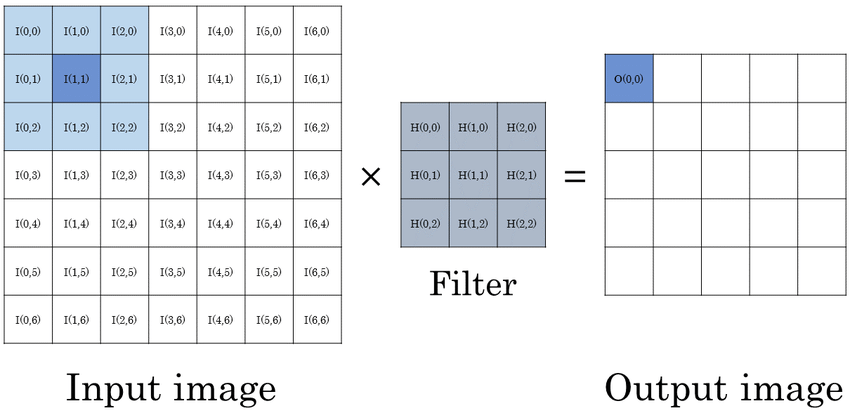
\includegraphics[width=1\linewidth]{figures/ImageConvolution.png}
	\caption{Image convolution \cite{fpgabasedCnovolution}}
	\label{fig:image convolution}
\end{figure}

\subsection{image blurring}
Image blurring is a frequently used image processing technique. The field of application lies in pre-processing for other image processing algorithms, such as feature extraction or edge detection. Image blurring is used as a filter to suppress noise. In this application, a 3x3 Gaussian kernel \ref{m:gausiankernel} is used as a blurring filter, the use of a division by 16 was dispensed. The kernel was applied using convolution.

\begin{center}
\begin{bmatrix}
1 & 2 & 1 \\
2 & 4 & 2 \\
1 & 2 & 1
\end{bmatrix}
\label{m:gausiankernel}
\end{center}

According to Table \ref{tab:perfBlurrEdge} the proposed adders have an an \gls{ssim} over 0.9 and \gls{psnr} of over 30 db, indicating a acceptable image quality. With five or more approximated bits this quality metrics could not be hold.
Figure \ref{fig:blurr1of8} to \ref{fig:blurr4of8} show the results for approximated image blurring algorithm. 

\begin{figure}[!htb]
	\centering
	\subfloat[]{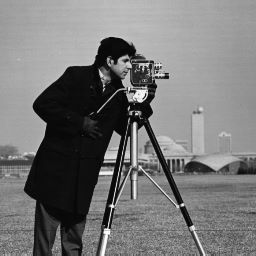
\includegraphics[width=0.3\linewidth]{figures/cameraman.jpg}}\label{fig:blurroriginal}\hfill
	\subfloat[]{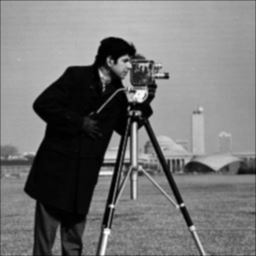
\includegraphics[width=0.3\linewidth]{figures/blurring_exact Serial [1]_1.png}\label{fig:blurrexact}}\hfill
	\subfloat[]{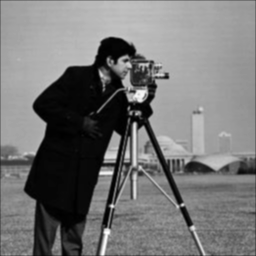
\includegraphics[width=0.3\linewidth]{figures/blurring_own Aprox [11]_1.png}\label{fig:blurr1of8}}\hfill
    \subfloat[]{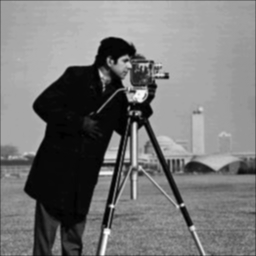
\includegraphics[width=0.3\linewidth]{figures/blurring_own Aprox [11]_3.png}}\label{fig:blurr3of8}\hfill
    \subfloat[]{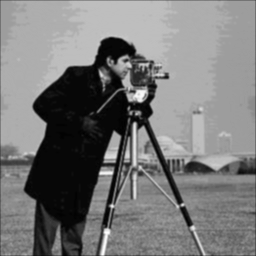
\includegraphics[width=0.3\linewidth]{figures/blurring_own Aprox [11]_4.png}}\label{fig:blurr4of8}\hfill
    \caption{Results of image blurring with different approximation degrees (a) cameraman original picture, (b) correct, (c) Ax 1/8, (d) Ax 3/8, (e) Ax 4/8}
\end{figure}

\subsection{edge detection}
Edge detection is a fundamental image processing technique it is widely used to identify the boundaries of objects within an image. The edges represent significant color or intensity changes. The process of edge detection is done by applying a convolution with a here chosen 3x3 sobel x kernel \cite{CHANG2023160}. In order to use the sobel x kernel, a twos complement algorithm was integrated resulting to perform bitwise addition and subtraction on base of the same logic table.

\begin{center}
\begin{bmatrix}
-1 & 0 & 1 \\
-2 & 0 & 2 \\
-1 & 0 & 1
\end{bmatrix}
\label{m:sobelxkernel}
\end{center}

Table \ref{tab:perfBlurrEdge} show the performance metrics for the proposed 8-bit \gls{rca}. It can be seen that for the proposed adders only the Ax 2/8 Adder is slightly below the threshold of 30dB. Ax 5/8 to 8/8 can not surpass this threshold.
Figure \ref{fig:edges1of8} to \ref{fig:edges4of8} show the results for the proposed adders.

\begin{figure}[!htb]
	\centering
	\subfloat[]{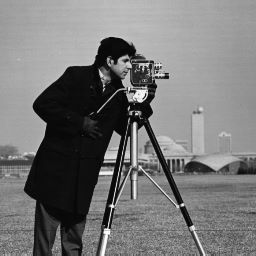
\includegraphics[width=0.3\linewidth]{figures/cameraman.jpg}}\label{fig:edgeoriginal}\hfill
	\subfloat[]{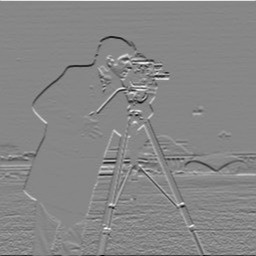
\includegraphics[width=0.3\linewidth]{figures/edge_exact Serial [1]_1.png}\label{fig:edgeexact}}\hfill
	\subfloat[]{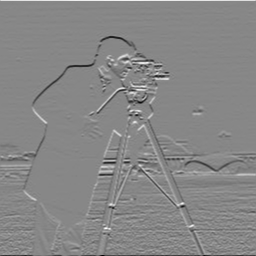
\includegraphics[width=0.3\linewidth]{figures/edge_own Aprox [11]_1.png}\label{fig:edges1of8}}\hfill
    \subfloat[]{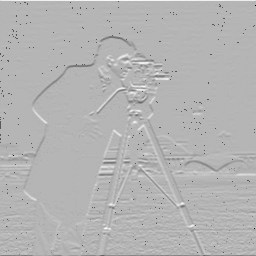
\includegraphics[width=0.3\linewidth]{figures/edge_own Aprox [11]_3.png}\label{fig:edges3of8}}\hfill
    \subfloat[]{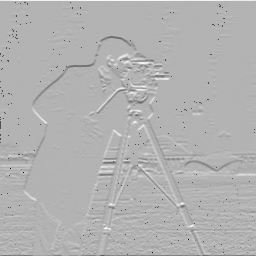
\includegraphics[width=0.3\linewidth]{figures/edge_own Aprox [11]_4.png}\label{fig:edges4of8}}\hfill
	\caption{Results of edge detection with different approximation degrees (a) cameraman original picture, (b) correct, (c) Ax 1/8, (d) Ax 3/8, (e) Ax 4/8}
	\label{fig:edge}
\end{figure}


\begin{table}[!ht]
\caption{quality metrics of image processing applications}
\centering
\begin{tabular}{|l|ll|ll|}
\hline
\multicolumn{1}{|c|}{\multirow{2}{*}{\begin{tabular}[c]{@{}c@{}}Approximated \\ Algorithm\end{tabular}}} & \multicolumn{2}{l|}{Image blurring} & \multicolumn{2}{l|}{edge detection}   \\ \cline{2-5} 
\multicolumn{1}{|c|}{} & \multicolumn{1}{l|}{SSIM} & PSNR (dB) & \multicolumn{1}{l|}{SSIM} & PSNR (dB) \\ \hline \addlinespace[1ex] \hline
Ax 1/8 & \multicolumn{1}{l|}{0.999} & 58.07 & \multicolumn{1}{l|}{0.990} & 58.25 \\ \hline
Ax 2/8 & \multicolumn{1}{l|}{0.998} & 45.5 & \multicolumn{1}{l|}{0.798} & 29.44 \\ \hline
Ax 3/8 & \multicolumn{1}{l|}{0.988} & 36.91 & \multicolumn{1}{l|}{0.776} & 31.99 \\ \hline
Ax 4/8 & \multicolumn{1}{l|}{0.966} & 30.26 & \multicolumn{1}{l|}{0.540} & 30.58 \\ \hline
\end{tabular}
\label{tab:perfBlurrEdge}
\end{table}

\begin{table*}[h]
\centering
\caption{Application comparison to exact Semi-Parallel Adder  \cite{8832255}}
\begin{tabular}{|c|cccc|cccc|}
\hline
\multirow{3}{*}{Algorithm} &
  \multicolumn{4}{c|}{image blurring (256x256 8-bit image)} &
  \multicolumn{4}{c|}{edge detection (256x256 8-bit image)} \\ \cline{2-9} 
 &
  \multicolumn{1}{c|}{\multirow{2}{*}{\begin{tabular}[c]{@{}c@{}}Energy/ \\ pixel (nJ)\end{tabular}}} &
  \multicolumn{1}{c|}{\multirow{2}{*}{\begin{tabular}[c]{@{}c@{}}Total \\ Energy (mJ)\end{tabular}}} &
  \multicolumn{1}{c|}{\multirow{2}{*}{\begin{tabular}[c]{@{}c@{}}Steps/\\ pixel\end{tabular}}} &
  \multirow{2}{*}{\begin{tabular}[c]{@{}c@{}}Total Steps\\ (million)\end{tabular}} &
  \multicolumn{1}{c|}{\multirow{2}{*}{\begin{tabular}[c]{@{}c@{}}Energy/\\ pixel (nJ)\end{tabular}}} &
  \multicolumn{1}{c|}{\multirow{2}{*}{\begin{tabular}[c]{@{}c@{}}Total \\ Energy (mJ)\end{tabular}}} &
  \multicolumn{1}{c|}{\multirow{2}{*}{\begin{tabular}[c]{@{}c@{}}Steps/\\ pixel\end{tabular}}} &
  \multirow{2}{*}{\begin{tabular}[c]{@{}c@{}}Total Steps\\ (million)\end{tabular}} \\
 &
  \multicolumn{1}{c|}{} &
  \multicolumn{1}{c|}{} &
  \multicolumn{1}{c|}{} &
   &
  \multicolumn{1}{c|}{} &
  \multicolumn{1}{c|}{} &
  \multicolumn{1}{c|}{} &
   \\ \hline \addlinespace[1ex] \hline
Semi-Parallel Exact {[}10{]} &
  \multicolumn{1}{c|}{222.86} &
  \multicolumn{1}{c|}{14.61} &
  \multicolumn{1}{c|}{2883.25} &
  188.96 &
  \multicolumn{1}{c|}{113.02} &
  \multicolumn{1}{c|}{7.41} &
  \multicolumn{1}{c|}{2008.32} &
  131.62 \\ \hline
Proposed (1/8) &
  \multicolumn{1}{c|}{202.95} &
  \multicolumn{1}{c|}{13.3} &
  \multicolumn{1}{c|}{2633.32} &
  172.58 &
  \multicolumn{1}{c|}{103.59} &
  \multicolumn{1}{c|}{6.79} &
  \multicolumn{1}{c|}{1851.22} &
  121.32 \\ \hline
Proposed (4/8) &
  \multicolumn{1}{c|}{145.37} &
  \multicolumn{1}{c|}{9.53} &
  \multicolumn{1}{c|}{1903.77} &
  124.77 &
  \multicolumn{1}{c|}{75.2} &
  \multicolumn{1}{c|}{4.93} &
  \multicolumn{1}{c|}{1374.99} &
  90.11 \\ \hline
\end{tabular}
\label{tab:imageAppComp}
\end{table*}

\subsection{Application-level comparison}
\subsubsection{Using Exact Semi-Parallel Adder \cite{8832255}}
To effectively compare our algorithm with the exact approach \cite{8832255}. We compared the \gls{rca} with 1/8 and 4/8 with the exact 8 Bit adder. Comparing the energy per pixel for exact version and proposed Adders, we see a energy reduction of 9\%-35\% and 9\%-34\% fewer steps, while the accuracy is still acceptable as show in Table \ref{tab:perfBlurrEdge}. We were able to save up to 5.8 mJ of energy and up to 64.19 million steps for an 256x256 8-bit image. An overview of the improvements can be seen in Table \ref{tab:imageAppComp} for image blurring and edge detection.
\subsubsection{Using different approximated adders}
To effectively compare our approximated adder and its metrics with other approximated adders, we compared our approximated adder against other published adders. It turns out that our algorithm can keep up with the other published algorithms in the metrics \gls{ssim} and \gls{psnr}. In terms of performance, it ranks below SIAFA1-3, but above SIAFA4 and serial approx. In terms of energy and steps, our proposed algorithm is among the best. 
Figure \ref{fig:blurrSSIMPSNRComp} and \ref{fig:edgeSSIMPSNRComp} show the comparison of \gls{ssim} and \gls{psnr} for image blurring and edge detection between multiple different approximation adders and our proppsed version.

\begin{figure}[h]
	\centering
	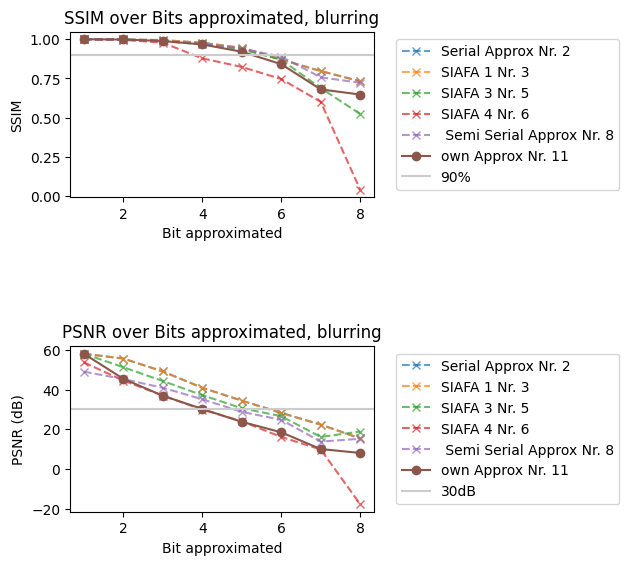
\includegraphics[width=0.85\linewidth]{figures/blurringSsiMPSNR.png}
	\caption{comparison of different approximation algorithms in image blurring application}
	\label{fig:blurrSSIMPSNRComp}
\end{figure}

\begin{figure}[h]
	\centering
	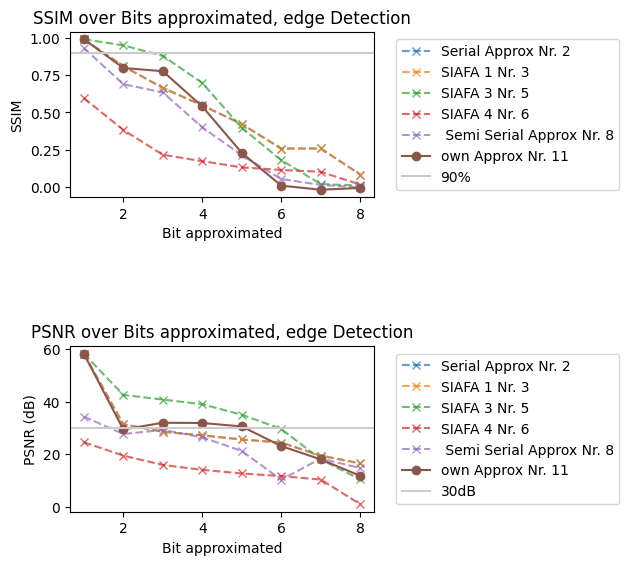
\includegraphics[width=0.85\linewidth]{figures/edgeDetectionSsiMPSNR.png}
	\caption{comparison of different approximation algorithms in edge detection application}
	\label{fig:edgeSSIMPSNRComp}
\end{figure}
%TODO: Conclusion, video, Wahrheitstabelle part schreiben 
%%% Florian Ende

\newpage

%%% Constantin Anfang
\section{Application in machine learning}
\label{ch:APPML}

\subsection{Choice of the network architectures}
Let me start this section of with some insights into the choice of the two network architectures. Both studying far more complex network architectures and examining more basic approaches like an MLP would have had its advantages. Insights into transformer networks would be far more easily applicable to the threatening real world energy consumption of large language models which might be alleviated through appropriate application of approximate computing techniques, especially with some kind of accuracy fragility measure checking for a good approximation level. Studying an MLP on the other hand would significantly decrease the problems complexity and allow for a more in detail study of the impact of the approximation. But while an MLP is simpler to design and implement, it also provides a lower computational intensity compared to any convolution based architecture. Therefore is makes less sense to optimise its computational component, while the memory intensity stays unchanged.\\
These considerations led to the choice of two network architectures mainly consisting of convolutional layers. When comparing the computational intensity of fully connected layers and convolutional layers the main difference stems from the fact that a fully connected layer needs $ N \cdot N$ weights with $N$ being the number of activations in the layers connected by the weights. In a convolutional layer on the other hand, the number of weights and thereby the memory cost is independent from the the layer dimensions and is only determined by the kernel dimensions which tend to be much smaller. This can be seen in the most common kernel size which is $ 3 \cdot 3$. This kernel size has become so common that is almost seems like a natural constant, but of course there are exceptions.\\
The other determining factor for the choice was the ubiquity and scalability from little edge processors to big accelerator farms which shows what versatile tool they are. They are a well proven part of the machine learning landscape and often the go to choice for a classifier.

\subsection{Tensorflow Approach}
The first approach I explored in order to simulate our memristor hardware in a machine learning application, was to comb through Tensorflow documentation and back end in order to find a way to implement a custom operator or layer. But while I gained more respect for the complexity of such a mature machine learning framework I also learned that it was beyond my abilities to edit its back end. I believe the Tensorflow back end is primaririly implemented in C++ and CUDA, which means I would have had to recompile the framework with the added or modified operators, which seemed to be beyond the scope to me.

\subsection{Only Inference No Training}
With the experience from the Tensorflow attempt I decided to implement the necessary functions to build the network myself. This resulted in the choice to only simulate inference and not try to build a whole training stack with back propagation, drop out and learning rate adjustment. Traditionally energy and time at most scarce at inference time, e.g. when used in some kind of user application on edge on a battery powered device instead of at training time in a data center. Therefore the possible savings from an approximate computing approach would be most effective here. \\
In light of the fact that I had no ability to train in my setup, I decided that the effort of copying pretrained weights from a different implementation, if ones with the correct dimensions are even available would not be worth it. I therefore did not measure any accuracy results. Without training these accuracy results would be in the best case misleading and in the worst case useless. Even with pretrained weights, I believe the actual learnings would lie in retraining for a few epochs to allow the network to adjust. This way it could adjust its weights to account for the weights and activations quantization and also adjust to the errors introduced by the approximate adder in use and possibly compensate to some degree. \\
In the given setting I have settled for measuring the next most important metric after the computational result. And since we have hit the energy wall on all scales from embedded system to data center, that metric is energy consumption and in concurrency with that also energy dissipation.

\subsection{Quantization}
In this project we have chosen int8 as out data type of choice. And while this is not a bad thing in itself, it necessitates a little deep dive into neural network quantization. Most basic neural networks operate with float32 as their main data type. And while the value range of float32 is not infinite, the range of $[-3.4028 \times 10^{38}, 3.4028 \times 10^{38}]$ dwarfs the one of int8 $[-128, 127]$. \\
The common approach would be to train the network in float32 and then quantize the weights and activations. The smaller the data type we a quantizing to the more challenging this step is. In order to do this, the maximum values that occur in the activations are measured and used as the maximum value in the quantized version. All activations are scaled accordingly. This approach does have a fatal flaw for smaller data types. It is not uncommon for a neural network to contain one or a few outlier values that are much larger then all others but might not be of significance to result due to dropout or some other effect. If we simply scale accordingly to this outlier, we give up a lot of valuable range in order to preserve it fully, while squeezing the rest of our network into an even smaller value range. This results in a very low resolution and can negatively impact accuracy. Therefore another common approach is clipping. The idea behind clipping is to set all values that would exceed the value range to some threshold value. These values are commonly the maximum and minimum value of our datatype. This does result in some information loss and can also negatively impact network accuracy, if the clipping cuts away outliers that carry information important to the network. Because we have this trade-off between information loss and resolution loss a combined approach is the optimum. The most thorough approach would be to quantize the network for all possible clipping tresholds and then scale with the clipped values. In order to find the correct threshold one would simply have to measure the accuracy for all values. The drawback of the approach is how expensive it is. In order to capture a meaningful accuracy value every threshold value testes would require a few epochs of retraining after quantization. This investment in training time can absolutely be worth it, e.g. when training a model that will be deployed to a large number of people that will run inference on it very often. In this case paying the extra training energy once seems like a good idea. \\
Because in our implementation there is no training, we have to start from the ground up in 8bit. We neither have pretrained values, nor do we have to rescale them to the 8bit value range. We do however still need to deal with the problem of exploding activations. Exploding activations are caused when the activation function, in our case ReLu, sets all negative values to zero and the convolutions adds up more and more larger and larger integers. This introduced a problem where we quickly run into activatations which would exceed our range. I therefore have implemented upper-bound clipping in the "SunnyMyWrapper" function ensuring we stay in the given 8bit value range.\\
It is likely that a more complex implementation could have alleviated this problem in a more elegant way. In a future work which would also allow for training I would expect the training to result in learned smaller weights which could keep the activations in check. Furthermore techniques such as dropout and batch normalization could also help in combating this behaviour. In dropout for each pass a random subset of neurons and connections is set to zero, in that sense dropped out of the network. This would certainly result in smaller sums. Batch normalization would not necessarily result in smaller values, but the normalization would keep outliers in check and outliers are what normally causes activation explosions. 

\subsection{Convolution}
The biggest challenge for the machine learning application was building a correctly functioning multi-channel convolution with stride and padding. This kind function is normally provided by the machine learning framework, e.g. Tensorflow but in order to incorporate our custom adder into the additions and multiplications it was written from scratch. \\
In the first step the number of input channels is determined for use in the computational kernel. The input image is padded in a channel-wise manner and the output map is initialized with all zero entries. The shape of the output map is determined by the input image dimensions and the kernel dimensions. \\
The two outer most loops of the computational kernel serve to extract the region of interest from the padded input image according to the set stride. This implementation only supports a stride of 1 or 2. This choice was sufficient for the desired network architectures and allowed for an implementation of division through bit-shift demonstrating the possibility of a  far more efficient implementation in hardware then a fully fledged division could offer. \\
Within the extracted region of interest there are four further loops which make up the actual convolution operation. The outer most one loops through the output channels to write the results into the correct output map channel. The next two loops go over height and width of the kernel. The inner most loop moves through the input channels. This step in the convolution connects the different layers and allows for layer transcending pattern recognition. In this innermost loop we use the custom addition and derived custom multiplication to perform the convolution operation.\\
The motivation for having a true multi-channel convolution was to be able to recreate real-world network architectures. In these architectures a variable number of input and output channels is used to change the dimensionality of the activations on order to move from wide feature maps with few channels to narrow feature maps with many channels. This kind of reversing funnel architecture allows for large input maps with a large number of channels deeper in the network, which can also serve as separate feature extractors and is used in both our implemented examples. 

\subsection{Skip Connections}
The last detail of the implementation worth mentioning are the skip connections in use in the ResNet. The are what sets a ResNet apart from a conventional convolutional net. \\
The invention on skip connections was caused by the problem on vanishing gradients. Vanishing gradients started to occur more and more with deeper networks. They are caused by gradients becoming exponentially smaller with layer number during backpropagation which can lead to slowed down or even stalled learning. \\
The idea behind a skip-connection is in principle the same as the one behind a bypass road. In order to avoid a stall we create a connection bypassing a number of layers. From the perspective of the backpropagation this cuts the network depth down by a factor of skip length and therefore helps avoiding vanishing gradients. These improved learning dynamics were a major step forward for convolutional nets because they made training significantly easier.\\
In our implementation these skip-connections were slightly modified in order to combat the afore-mentioned activation explosion. They now do not only add the feature maps of the current layer and an earlier one, but they also regularize the sum to a maximum of 100 in order to comfortably remain in the int8 value range. Otherwise these additions lead to an accelerated activation explosion which then leads to information loss due to clipping. 

\begin{figure}[h]
  \centering
  \includesvg[width=0.4\textwidth]{figures/resnet.svg} 
  \caption{This figure shows the implemented ResNet archtitecture. Only the first layer convolution is 5x5, while all following ones are 3x3 convolutions. The last layer is a fully connected layer. On the right side the skip-connections are shown. It can be seen that the skip-connections are always only within one block of the same dimensions, since the addition of feature maps of different dimensions is not possible.}
\end{figure}

\subsection{ResNet}
The ResNet can injest an input image of arbitrary dimensions and an arbitrary number of input channels. We would however normally expect three input channels for the RGB values of an image. Its architecture follows the reversing funnel paradigm, but employs skip-connections within each block of similarly shaped convolutions. The down-sampling to a smaller feature map at each block edge is achieved using a stride of two and the kernel dimensions widen the number of channels at the same time.  The network consists of 15 layer. Fourteen of these layers are convolutional layers, the last one before the softmax which provides the output probabilities is a fully connected layer. It also contains a total of six skip-connections. 

\begin{figure}[h]
  \centering
  \includesvg[width=0.4\textwidth]{figures/convnet.svg} 
  \caption{This figure shows the implemented plain convolutional net architecture. Here the shrinking of the feature map is not achieved through block-wise stride two layers, but instead the padding and kernel size are chosen to result in a gradual shrinking of the feature map. Once the switch to 32 channels happens the feature map size is held constant. }
\end{figure}

\subsection{Convolutional Net}
The convolutional net has a pretty similar basic architecture to the ResNet, but it does not contain skip-connections. Additionally it employs a stronger widening of the channel number going to 32 channels for four layers before one last 64 channel convolutional layer. The ResNet on the other hand has a maximum of 24 channels. For both ResNet and convolutional net the number of output classes is set arbitrarily to ten, but could be modified to fit any classification workload. Instead of achieving a shrinking of the feature map dimensions through the means of layers with stride two, the reduction is achieved through the relationship of padding and kernel size. These are chosen to shrink the feature map dimensions down to a minimum value before the switch from 6 to 32 channels happens. From there on out the feature map dimensions stay constant until the final fully connected layer. 

\begin{figure}[h]
	\centering
	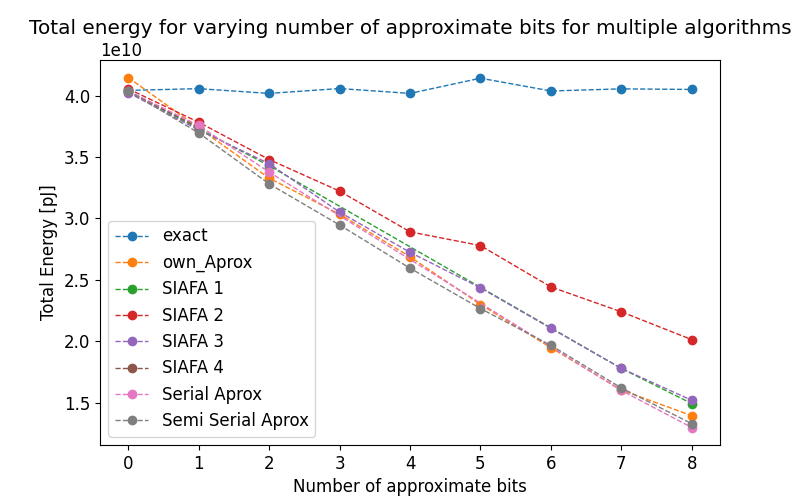
\includegraphics[width=1\linewidth]{figures/resnet_new.png}
	\caption{ResNet measurement. This figure shows the total energy for all algorithms for zero to eight approximated bits. The roughly linear relationship between number of approximated bits and decrease in energy consumption is apparent for all approximate algorithms. Our own approximate algorithm shows performance similar to the best approximate algorithms from this sample in terms of energy efficiency.}
	\label{fig:resnet_energy}
\end{figure}

\begin{figure}[h]
	\centering
	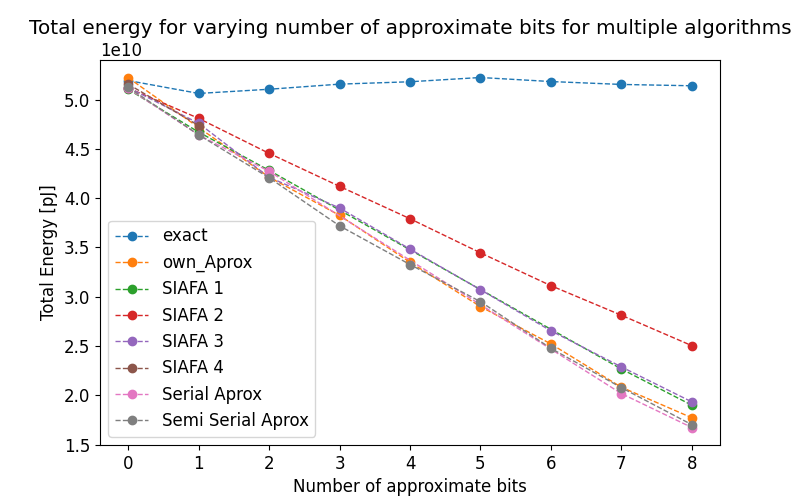
\includegraphics[width=1\linewidth]{figures/convnet_new.png}
	\caption{Plain convolutional net measurement. This figure shows the total energy for all algorithms for zero to eight approximated bits. The behaviour resembles the one observed for the ResNet. It differs in absolute energy, which is explained by the computationally more expensive wider channels in this net.}
	\label{fig:resnet_energy}
\end{figure}


\begin{figure}[h]
	\centering
	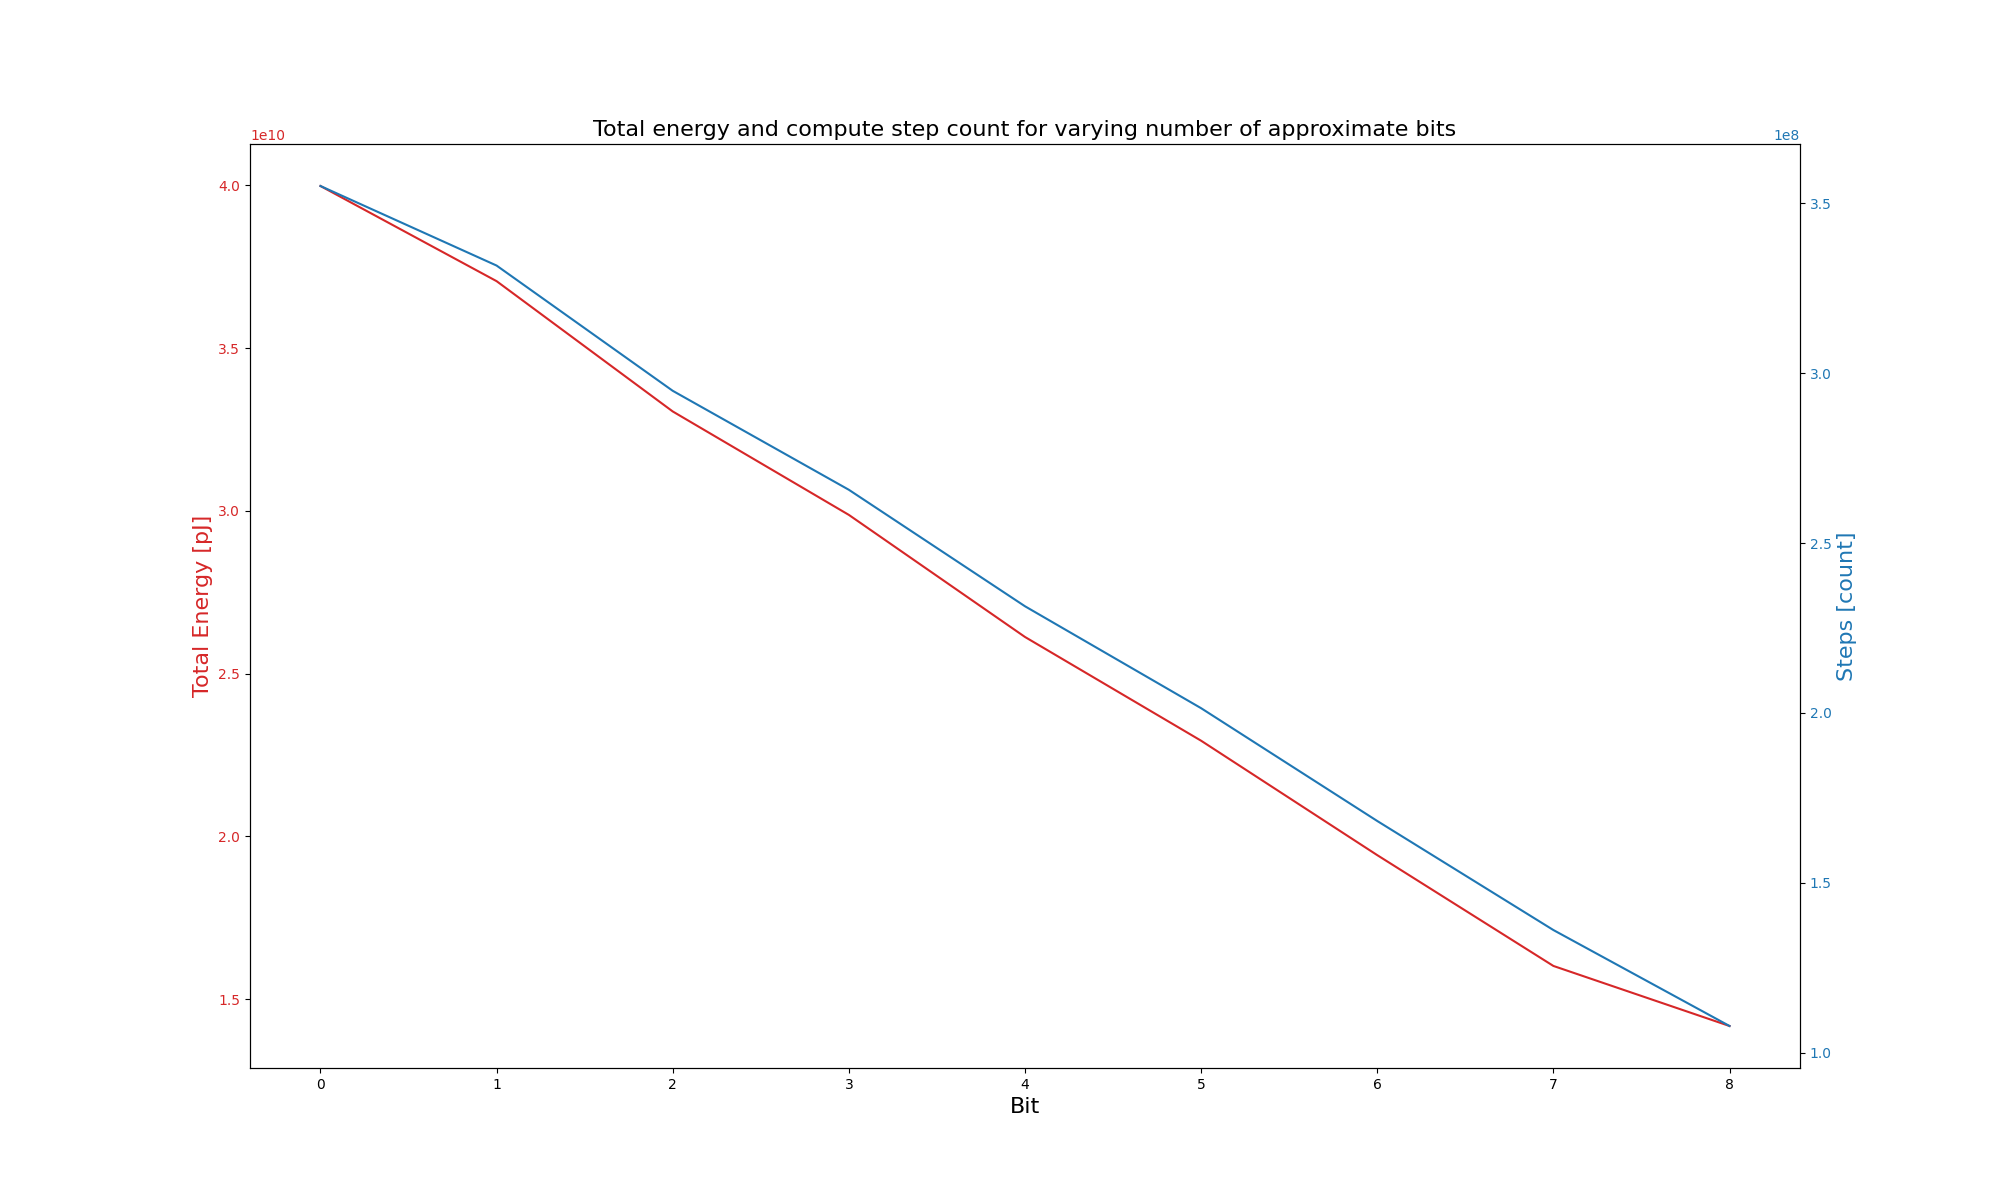
\includegraphics[width=1\linewidth]{figures/stepsplot.png}
	\caption{This figure shows the energy consumption and the step count for zero to eight bits approximated with our own approximate adder algorithm. Both show a linear decrease with more approximate bits which is expected behaviour. These measurements were performed on the ResNet model architecture.}
	\label{fig:resnet_energy}
\end{figure}


\subsection{Energy and Step Count Results}
To gather the results for the energy consumption of all algorithms at all approximated bit widths, a run of each scenario was performed. All measurements were conducted on the same test image, but the weights were randomly initialized for each run. This is most likely the cause of the small deviations in the exact run for different bit widths. It also explains small differences in the measurements for all algorithms with zero approximated bits. These statistical fluctuations could have been eliminated by running the measurement multiple times, but the computational costs of the simulation were prohibitively high. Therefore one run was deemed sufficient to gain a general insight. \\
The plot of the ResNet energy measurement results shows all approximate algorithms performing significantly better than the exact adder in terms of energy efficiency. And while the SIAFA 2 algorithms performs a little worse than the others the rest is packed pretty close together. In fact I can confidently state that our algorithm performs comparably well to the best algorithms from our sample set in terms of energy efficiency. We can observe a linear decrease in energy consumption with each added approximate bit to the adder. This an exponential decrease would have been more exciting, the benefit of a linear relationship is, that we do not need to go to a large number of approximate bits to already gain the advantage of our custom adder. Even approximating only two or three bits will already result in significant energy savings. \\
The plot for the plain convolutional net tells a very similar story. The most significant observable difference is the absolute difference in total energy consumption. This is caused by the wider channels towards the end of the plain convolutional net, which are computationally more intensive. \\
The comparison of energy consumption and step count for our own approximate adder displays a similar trend for both energy and step count. The step count too decreases linearly with more approximated bits. It does seem apparent though, that the energy consumption falls of at a slightly steeper angle than the step count. Although this slight difference does not appear to be significant to me and could simply be caused by statistical noise, it could be caused by a larger number of lower order bits which are already approximate resulting in higher order bit additions which happen to be a cheap to add combination of bits in our adder. If this dynamic is at play it could explain the slightly differing angles. 




\subsection{Outlook}
The search for a more efficient neural network implementation for inference through unsafe optimizations is not a new endeavor. Approaches such as quantization and pruning are widely used and regarded as the go to way to increase network efficiency. In this context one tool which is used to achieve this goal is Galen, which was developed by colleagues from ZITI. This tool operates by scanning the multi-dimensional search space of quantization and pruning possibilities in order to find the most efficient and performant combination. I propose expanding on this tool and extending the search space to include the optimal number of approximate bits in a for a custom more efficient adder. This way an over approximation can be avoided, since it would likely be more efficient to employ less drastic approximations in terms of quantization and pruning. \\
My only concern is that it might be prohibitively expensive to introduce another dimension into the search space, but this would require further investigation to determine. And even if today's computational resources are not sufficient, maybe the ones of tomorrow are. 

%%% Constatntin Ende

\section{Conclusion}
A new approximated RCA has been presented in this version. The functionality is based on memristors and their IMPLY-logic based functionality. We focused on reduction of energy and computational steps. As shown in privious parts we achieved an energy reduction of up to 35\%, for the metric of computational steps we achieved a reduction of up to 34\%, with comparable results in accuracy. We checked the functionality and correctness using LTSPICE and Python simulations. The technical application was demonstrated using two applications in image processing and machine learning. Our results show that the four-bit approximator shows an acceptable \gls{psnr} for the applications shown.

%%%%%%%%%%%%%%%%%Erklärungen zum Anhang                                 %%%%%%%%%%%%%%%%%%%%%%%%%%%%%%%%%
\clearpage
\section{Attachments}

\begin{table}[h]
\centering
\caption{}
\label{tab:attachments}
\begin{tabular}{|l|l|l|}
\hline
 & File name & Description \\ \hline
 \addlinespace[1ex] \hline
1 & LTSpice\_semiparallel\_SPAFA5\_8bit3apprx\_v01 & \begin{tabular}[c]{@{}l@{}}LTSpice simulation file for an 8-bit semi-parallel adder.\\ Input files for an 8-bit addition with the first \\ 3 bits \textbf{approximated} and the last 5 bits calculated \textbf{exactly}.\end{tabular} \\ \hline
2 & LTSpice\_semiparallel\_Adder4bitExact\_v01 & \begin{tabular}[c]{@{}l@{}}LTSpice simulation file for a 4-bit semi-parallel adder.\\ Input files for a 4-bit \textbf{exact} addition.\end{tabular} \\ \hline
3 & LTSpice\_semiparallel\_Adder1bitExact\_v01 & \begin{tabular}[c]{@{}l@{}}LTSpice simulation file for an 1-bit semi-parallel adder.\\ Input files for an 1-bit \textbf{exact} addition.\end{tabular} \\ \hline
4 & LTSpice\_semiparallel\_SPAFA5\_Adder1bitApx\_v01 & \begin{tabular}[c]{@{}l@{}}LTSpice simulation file for an 1-bit semi-parallel adder.\\ Input files for an 1-bit \textbf{approximating} addition.\end{tabular} \\ \hline
5 & LTSpice\_semiparallel\_SPAFA5\_Adder4bitApx\_v01 & \begin{tabular}[c]{@{}l@{}}LTSpice simulation file for a 4-bit semi-parallel adder.\\ Input files for a 4-bit \textbf{approximating} addition.\end{tabular} \\ \hline
6 & resources folder  & all the nessesary pictures \\ \hline
7 & 8Bit_qualitymetrics.ipynb & file for calculating quality metrics \\ \hline
8 & 8BitRCA.json & dictionary with all the calculated values \\ \hline
9 & calculationScript.py & Script for calculating all the pictures in a time efficient way\\ \hline
10 & data.json & dictionary with truthtable, steps and energy  calculationScript.py  \\ \hline
11 & datavisualization.ipynb & drawing plots and visualize data created by  calculationScript.py \\ \hline
12 & results.json & dictionary with all the calculated quality metrics from calculationScript.py\\ \hline
\end{tabular}
\end{table}

%%%%%%%%%%%%%%%%%Hier beginnen die Hinweise zum Umgang mit dem Template %%%%%%%%%%%%%%%%%%%%%%%%%%%%%%%%%
\clearpage
\section{How to use?}
This is just a template project. If you receive a copy of it, feel free to use as fits your purpose. If you have access to the original template file (\red{That is almost never the case}), do not write here or change parts of the original template randomly. Recommendation is to use a copy of setup file and edit the local version for your own use and \blue{link the acronyms and bib files} to your project (and add/edit the original acronym file here). 

If you add items to the acronyms or bib files (that are not there yet), please make sure you follow the respective instructions (add in appropriate section in \green{ALPHABETICAL ORDER}).\\





Generally, if you plan to make any adjustment or improvement here in the template file (especially in the setup), please make sure you do it properly; e.g., add items to relevant sections, in ALPHABETICAL ORDER, use proper versioning (especially if you are tweaking redaction and document appearance mode) and create a copy of previous versions accordingly.\\

\nima{If I have made a comment requiring an action, the best way is to write another comment replying what you did for it or that you have done it and it's finished (a simple ``Done'' or ``Okay'' is often sufficient). Removing my comment because you think you have applied it, makes it harder for me to check and takes a longer time.}

An example of using redactions and alternative texts is redacted because it was ``uncritical''.


\begin{Uncritical}
Example of alternative text is that right now is
\begin{TextA}
Day
\end{TextA}
\begin{TextB}
Night
\end{TextB}
, and that depends on the value of alttextmode variable in the beginning.
\end{Uncritical}

\section{Examples}

\begin{figure}[!bth] % Priority to place the figure: b=Bottom, t=Top, h=Here
%\vspace{-4mm}  % To reduce the (vertical) space between the figure and the text to a value smaller than the default
\centering
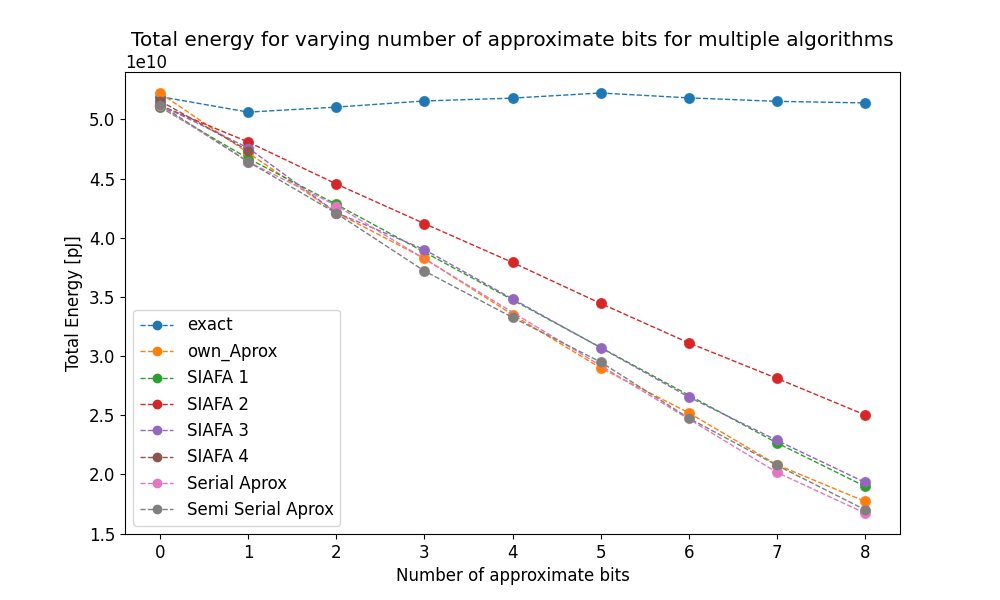
\includegraphics[width=0.96\columnwidth]{sample}
\caption{Here goes the caption.}
\label{fig_sample}
%\vspace{-4mm}  % To reduce the (vertical) space between the figure and the text to a value smaller than the default
\end{figure}
A sample figure can be seen in \Cref{fig_sample}.

\begin{figure}[!bth] % Priority to place the figure: b=Bottom, t=Top, h=Here
%\vspace{-4mm}  % To reduce the (vertical) space between the figure and the text to a value smaller than the default
\centering
\subfloat[first \label{fig_subfigure_one}]{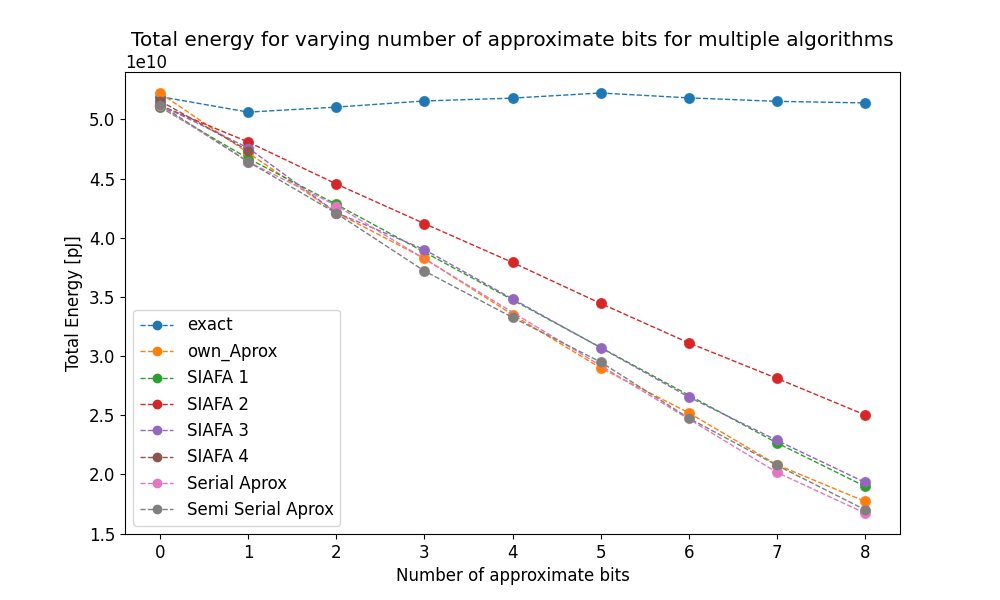
\includegraphics[width=0.46\columnwidth]{sample}}
\hfill
\subfloat[second \label{fig_subfigure_two}]{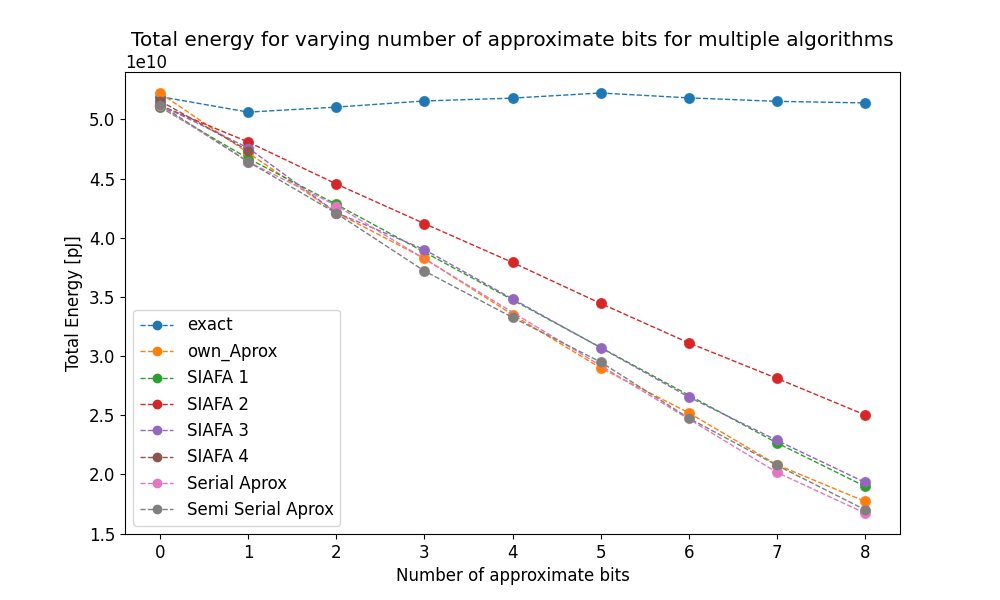
\includegraphics[width=0.46\columnwidth]{sample}}
\caption{A sample of a figure with subfigures.}
\label{fig_subfigure}
%\vspace{-4mm}  % To reduce the (vertical) space between the figure and the text to a value smaller than the default
\end{figure}

Citation~\cite{Taherinejad2016_CompObs}, \cite{anzanpour:2017a}.

\begin{table}[!tbh]
    \centering
    %\tiny
    \caption{Caption}
    \label{tab:my_label}
    
    %\begin{adjustbox}{width=\textwidth}
    \begin{threeparttable}
    \begin{tabular}{|c|c c c | c|}
         \hline
         \multirow{2}{*}{Multirow}  & \multicolumn{3}{c|}{Multicolumn} & 1\\
         \cline{2-5}
          & 2 & 3 & 4 & 5\textsuperscript{+} \\
         \hline \hline
         6 & 7 & 8 & 9 & 10 \\
         11 & 12\textsuperscript{*} & 13 & 14 & 15 \\
         \hline
    \end{tabular}
      \begin{tablenotes}
       %\scriptsize
       \item[+] Percentage of improvement (Imp.) is calculated based on $n \to \infty$.
       \item[*]$c=8$ for all calculated $FoM_A$.
     \end{tablenotes}
     \end{threeparttable}
     %\end{adjustbox}
     %\Vspace{-1mm}
\end{table}

To have an equation that spans across two columns you can \Cref{equ:S_{AND,q,p}}.
\begin{figure*}[!tbh]
% https://tex.stackexchange.com/questions/16429/equation-spanning-two-columns-in-ieeetran
	\begin{align}
	S_{\texttt{AND},q,p}[i] &= \left\{ \begin{array}{llr} 
		\text{1} &\{ nx +q\cdot vn+p\cdot v \le i < kx+q\cdot vn+(p+1)\cdot v\} \text{ for } x<v &(\text{a})\\
		\text{1} &\{ k(x+1)+q\cdot vn+p\cdot v \le i < nx+q\cdot vn+(p+1)\cdot v\} \text{ for } x>k-v &(\text{b})\\
		\text{0} &\text{else} &(\text{c})
		\end{array} \right. 	\label{equ:S_{AND,q,p}}
		\end{align}
\end{figure*}



%\newpage
%\IEEEtriggeratref{14}
\bibliographystyle{IEEEtran}
%\bibliography{unsrt}
%\bibliographystyle{setups/unsrt2authabbrvpp}    % Automatic truncating of authors' list for unsrt package (for IEEE template and cite package check in the "reference.bib" the \bstctlcite{IEEEexample:BSTcontrol}. That is, uncomment that command after the \begin{document}. )
%\bibliographystyle{acmtrans}
%\bibliographystyle{ACM-Reference-Format}
\bibliography{references,setups/nima,setups/memristor_lit}

% \begin{IEEEbiography}
% [{\includegraphics[width=1in,height=1.25in,clip,keepaspectratio]{figures/Nima_TaheriNejad.jpg}}]{Nima TaheriNejad} (S'08-M'15) 
% \input{setups/nima-bio.tex}
% \end{IEEEbiography}

% \begin{IEEEbiographynophoto}{NoPhoto}
% Manuscripts accepted for publication should be accompanied by a brief biographical sketch for each author. Biographical information should include only the following information: Current title or position, up to three research interests, highest academic degree, discipline in which the degree was awarded, granting institution, membership in relevant professional societies (such as the IEEE Circuits and Systems Society and the ACM), and e-mail address.
% \end{IEEEbiographynophoto}

\end{document}
